\documentclass{article}
\usepackage{graphicx}
\usepackage{amssymb,amsmath}
\usepackage{tikz}
\usepackage{pgfplots}
\pgfplotsset{compat=newest}
\pgfplotsset{plot coordinates/math parser=false}
\newlength\figureheight
\newlength\figurewidth
\usetikzlibrary{shapes, arrows, patterns}
\usetikzlibrary{external}
\tikzexternalize[shell escape=-enable-write18]
\tikzset{external/system call={lualatex \tikzexternalcheckshellescape -halt-on-error -interaction=batchmode -jobname "\image" "\texsource"}}
\tikzset{external/force remake}

\DeclareRobustCommand{\BlackBox}{\State \textbf{Black Box: }}
\DeclareRobustCommand{\Test}{\State \textbf{Test: }}
\DeclareRobustCommand{\Define}{\State \textbf{Define: }}
\DeclareRobustCommand{\Update}{\State \textbf{Update: }}
\DeclareRobustCommand{\Set}{\State \textbf{Set: }}
\DeclareRobustCommand{\Calculate}{\State \textbf{Calculate: }}
%\newcommand{\algorithmicset}{\textbf{Set:}}
%\algnewcommand\Solve{\item[\algorithmicset]}
%============================================================================
% commands.tex
%============================================================================
% This file contains:
% 	- Defined Variables
%	- Redefined math shorthand
%	- Defined math shorthand


%============================================================================
% Redefined Math Commands
%============================================================================
% 	- \Vec{1} or \vec{1}
%		Long Name: Vector
%		Arguements[1]: bold and overbar arg1	
\DeclareRobustCommand{\Vec}[1]{%
    \ifmmode
        \mathbf{#1}\,%
    \else
        $\displaystyle \mathbf{#1}\,$%
    \fi
}
\DeclareRobustCommand{\vec}[1]{\Vec{#1}}

\DeclareRobustCommand{\lbm}{%
    \ifmmode
        \text{lb}_{\text{m}}
    \else
        $\displaystyle \text{lb}_{\text{m}}$%
    \fi
}
\DeclareRobustCommand{\lbf}{%
    \ifmmode
        \text{lb}_{\text{f}}
    \else
        $\displaystyle \text{lb}_{\text{f}}$
    \fi
}
\DeclareRobustCommand{\dt}{%
	\ifmmode
		\Delta t
	\else
		$\Delta t$
	\fi
}
\DeclareRobustCommand{\dtmax}{%
	\ifmmode
		\Delta t_{\text{MAX}}
	\else
		$\Delta t_{\text{MAX}}$
	\fi
}
\DeclareRobustCommand{\dx}{%
	\ifmmode
		\Delta x
	\else
		$\Delta x$
	\fi
}

\delimitershortfall-1sp
\newcommand\abs[1]{\left|#1\right|}

\tikzstyle{Decision} = [diamond, draw, text width=4.5em, text badly centered, node distance=3cm, inner sep=0pt]
\tikzstyle{Action} = [rectangle, draw,text width=5em, text centered, node distance=3cm, rounded corners, minimum height=0em]
\tikzstyle{NodePoint} = [circle, draw, minimum height = 0 em, node distance = 3 cm]
\tikzstyle{BlackBox} = [rectangle, draw, text centered, node distance=1cm, fill=black!10]
\tikzstyle{line} = [draw, -latex']
    

\begin{document}

\begin{figure}
\centering
% This file was created by matlab2tikz v0.4.3.
% Copyright (c) 2008--2013, Nico Schlömer <nico.schloemer@gmail.com>
% All rights reserved.
% 
\tikzsetnextfilename{plots/single1pt000em5_eps}
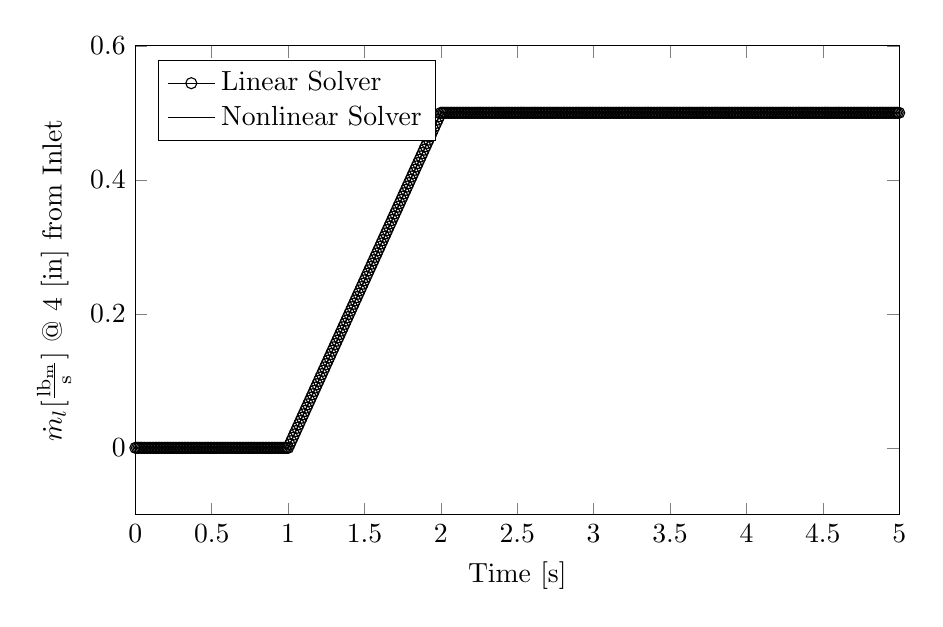
\begin{tikzpicture}

\begin{axis}[%
width=0.8\textwidth,
%height=0.630967741935484\textwidth,
height=0.491294629700995\textwidth,
scale only axis,
xmin=0.0,
xmax=5.0,
xlabel={Time $[\text{s}]$},
ymin=-0.1,
ymax=0.6,
ylabel={$\dot{m}_{l} [\frac{\lbm{}}{\text{s}}]$ @ 4 [in] from Inlet},
legend style={at={(0.03,0.97)},anchor=north west,draw=black,fill=white,legend cell align=left}
]
\addplot [
color=black,
solid,
mark=o,
mark options={solid}
]
table[row sep=crcr]{
0.0 0.0\\
0.0100024435669184 2.84913312498247e-05\\
0.020002443343401 6.3776082242839e-05\\
0.0300024431198835 6.68911525281146e-05\\
0.0400024428963661 5.20597714057658e-05\\
0.0500024445354939 3.02229072985938e-05\\
0.0600024424493313 8.62097022036323e-06\\
0.070002444088459 -8.08286313258577e-06\\
0.0800024420022964 -1.77508427441353e-05\\
0.0900024399161339 -2.0457244318095e-05\\
0.100002445280552 -1.77929214260075e-05\\
0.110002443194389 -1.20413887998438e-05\\
0.120002441108227 -5.4509541769221e-06\\
0.130002439022064 2.57638987477549e-07\\
0.140002444386482 4.09452377425623e-06\\
0.1500024497509 5.80263849769835e-06\\
0.160002440214157 5.68671612199978e-06\\
0.170002445578575 4.3527188609005e-06\\
0.180002436041832 2.48281412495999e-06\\
0.19000244140625 6.6041320678778e-07\\
0.200002446770668 -7.27347639895015e-07\\
0.210002437233925 -1.51257336256094e-06\\
0.220002442598343 -1.71384147051867e-06\\
0.230002447962761 -1.47271020978224e-06\\
0.240002438426018 -9.83303834800608e-07\\
0.250002443790436 -4.32722686127818e-07\\
0.260002434253693 3.80195892546453e-08\\
0.270002454519272 3.50443571051073e-07\\
0.280002444982529 4.8601015123495e-07\\
0.290002435445786 4.71122689305048e-07\\
0.300002455711365 3.56985424332379e-07\\
0.310002446174622 2.00401871097711e-07\\
0.320002436637878 4.94536074313601e-08\\
0.330002456903458 -6.43351896201239e-08\\
0.340002447366714 -1.27682696415832e-07\\
0.350002437829971 -1.42671197522759e-07\\
0.360002458095551 -1.21394094776406e-07\\
0.370002448558807 -8.00980686221919e-08\\
0.380002439022064 -3.4274272309176e-08\\
0.390002429485321 4.52052972832462e-09\\
0.4000024497509 2.9961800152023e-08\\
0.410002440214157 4.06867926017185e-08\\
0.420002430677414 3.90151591034282e-08\\
0.430002450942993 2.9264075607216e-08\\
0.44000244140625 1.61591167113784e-08\\
0.450002431869507 3.66112762328896e-09\\
0.460002452135086 -5.66451019423653e-09\\
0.470002442598343 -1.07697006868079e-08\\
0.4800024330616 -1.18717347064035e-08\\
0.490002453327179 -1.00023243021496e-08\\
0.500002443790436 -6.52047882354623e-09\\
0.510002434253693 -2.70829381143756e-09\\
0.520002424716949 4.87552886951903e-10\\
0.530002415180206 2.55794807557663e-09\\
0.540002465248108 3.40432459999818e-09\\
0.550002455711365 3.22969895272252e-09\\
0.560002446174622 2.39778930044565e-09\\
0.570002436637878 1.30157373767759e-09\\
0.580002427101135 2.67199290471254e-10\\
0.590002417564392 -4.96727770027405e-10\\
0.600002467632294 -9.0770491123493e-10\\
0.610002458095551 -9.87435577748386e-10\\
0.620002448558807 -8.23812018602155e-10\\
0.630002439022064 -5.30460286807255e-10\\
0.640002429485321 -2.13447412522605e-10\\
0.650002419948578 4.97134937382793e-11\\
0.660002470016479 2.18082135683417e-10\\
0.670002460479736 2.84695933494561e-10\\
0.680002450942993 2.6725097135305e-10\\
0.69000244140625 1.96373237115743e-10\\
0.700002431869507 1.04723278659957e-10\\
0.710002422332764 1.91418270123478e-11\\
0.720002472400665 -4.3403267091513e-11\\
0.730002462863922 -7.64486390858465e-11\\
0.740002453327179 -8.20911394416868e-11\\
0.750002443790436 -6.78251413366304e-11\\
0.760002434253693 -4.3130308352568e-11\\
0.770002424716949 -1.67756832730737e-11\\
0.780002415180206 4.87781343094795e-12\\
0.790002465248108 1.85687975412518e-11\\
0.800002455711365 2.3792990147542e-11\\
0.810002446174622 2.20966994701755e-11\\
0.820002436637878 1.6075077033384e-11\\
0.830002427101135 8.41679590607436e-12\\
0.840002417564392 1.34093940378638e-12\\
0.850002467632294 -3.7796458671191e-12\\
0.860002458095551 -6.43508987416275e-12\\
0.870002448558807 -6.81968760976592e-12\\
0.880002439022064 -5.58371838349503e-12\\
0.890002429485321 -3.50762257780857e-12\\
0.900002419948578 -1.31035438576121e-12\\
0.910002470016479 4.69463335393827e-13\\
0.920002460479736 1.57579049635259e-12\\
0.930002450942993 1.98898341373377e-12\\
0.94000244140625 1.82955430319542e-12\\
0.950002431869507 1.31339459707308e-12\\
0.960002422332764 6.75954463843359e-13\\
0.970002472400665 8.3715132536636e-14\\
0.980002462863922 -3.15176785494961e-13\\
0.990002453327179 -5.37747147158485e-13\\
1.00000238418579 2.53402081540344e-08\\
1.01000249385834 0.00498206028714776\\
1.02000248432159 0.00997622683644295\\
1.03000247478485 0.0149767594411969\\
1.04000246524811 0.0199822336435318\\
1.05000245571136 0.0249901637434959\\
1.06000244617462 0.0299980640411377\\
1.07000243663788 0.035004198551178\\
1.08000242710114 0.0400077626109123\\
1.09000241756439 0.0450087711215019\\
1.10000240802765 0.050007801502943\\
1.11000239849091 0.0550056844949722\\
1.12000238895416 0.0600032433867455\\
1.13000249862671 0.0650011226534843\\
1.14000248908997 0.0699996799230576\\
1.15000247955322 0.074999026954174\\
1.16000247001648 0.079999066889286\\
1.17000246047974 0.0849995687603951\\
1.18000245094299 0.0900002717971802\\
1.19000244140625 0.0950009748339653\\
1.20000243186951 0.100001506507397\\
1.21000242233276 0.10500180721283\\
1.22000241279602 0.110001891851425\\
1.23000240325928 0.115001797676086\\
1.24000239372253 0.1200016066432\\
1.25000238418579 0.125001385807991\\
1.26000249385834 0.130001202225685\\
1.27000248432159 0.135001078248024\\
1.28000247478485 0.140001028776169\\
1.29000246524811 0.145001038908958\\
1.30000245571136 0.15000107884407\\
1.31000244617462 0.155001133680344\\
1.32000243663788 0.160001203417778\\
1.33000242710114 0.16500124335289\\
1.34000241756439 0.170001268386841\\
1.35000240802765 0.17500127851963\\
1.36000239849091 0.180001273751259\\
1.37000238895416 0.185001254081726\\
1.38000249862671 0.190001234412193\\
1.39000248908997 0.195001214742661\\
1.40000247955322 0.200001209974289\\
1.41000247001648 0.205001205205917\\
1.42000246047974 0.210001200437546\\
1.43000245094299 0.215001210570335\\
1.44000244140625 0.220001220703125\\
1.45000243186951 0.225001215934753\\
1.46000242233276 0.230001226067543\\
1.47000241279602 0.235001221299171\\
1.48000240325928 0.240001231431961\\
1.49000239372253 0.245001226663589\\
1.50000238418579 0.250001221895218\\
1.51000249385834 0.255001217126846\\
1.52000248432159 0.260001212358475\\
1.53000247478485 0.265001207590103\\
1.54000246524811 0.270001232624054\\
1.55000245571136 0.275001227855682\\
1.56000244617462 0.280001223087311\\
1.57000243663788 0.285001218318939\\
1.58000242710114 0.290001213550568\\
1.59000241756439 0.295001208782196\\
1.60000240802765 0.300001233816147\\
1.61000239849091 0.305001229047775\\
1.62000238895416 0.310001224279404\\
1.63000249862671 0.315001219511032\\
1.64000248908997 0.320001214742661\\
1.65000247955322 0.325001209974289\\
1.66000247001648 0.33000123500824\\
1.67000246047974 0.335001230239868\\
1.68000245094299 0.340001225471497\\
1.69000244140625 0.345001220703125\\
1.70000243186951 0.350001215934753\\
1.71000242233276 0.355001211166382\\
1.72000241279602 0.360001236200333\\
1.73000240325928 0.365001231431961\\
1.74000239372253 0.370001226663589\\
1.75000238418579 0.375001221895218\\
1.76000249385834 0.380001217126846\\
1.77000248432159 0.385001212358475\\
1.78000247478485 0.390001207590103\\
1.79000246524811 0.395001232624054\\
1.80000245571136 0.400001227855682\\
1.81000244617462 0.405001223087311\\
1.82000243663788 0.410001218318939\\
1.83000242710114 0.415001213550568\\
1.84000241756439 0.420001208782196\\
1.85000240802765 0.425001233816147\\
1.86000239849091 0.430001229047775\\
1.87000238895416 0.435001224279404\\
1.88000249862671 0.440001219511032\\
1.89000248908997 0.445001214742661\\
1.90000247955322 0.450001209974289\\
1.91000247001648 0.45500123500824\\
1.92000246047974 0.460001230239868\\
1.93000245094299 0.465001225471497\\
1.94000244140625 0.470001220703125\\
1.95000243186951 0.475001215934753\\
1.96000242233276 0.480001211166382\\
1.97000241279602 0.485001236200333\\
1.98000240325928 0.490001231431961\\
1.99000239372253 0.495001226663589\\
2.00000238418579 0.500001192092896\\
2.01000237464905 0.500019133090973\\
2.0200023651123 0.500024974346161\\
2.03000235557556 0.500024378299713\\
2.04000234603882 0.500018894672394\\
2.05000233650208 0.500011026859283\\
2.06000232696533 0.500003159046173\\
2.07000255584717 0.499997049570084\\
2.08000254631042 0.499993503093719\\
2.09000253677368 0.499992519617081\\
2.10000252723694 0.499993473291397\\
2.1100025177002 0.499995589256287\\
2.12000250816345 0.4999980032444\\
2.13000249862671 0.50000011920929\\
2.14000248908997 0.500001549720764\\
2.15000247955322 0.500002145767212\\
2.16000247001648 0.500002145767212\\
2.17000246047974 0.500001609325409\\
2.18000245094299 0.500000953674316\\
2.19000244140625 0.500000238418579\\
2.20000243186951 0.499999731779099\\
2.21000242233276 0.499999433755875\\
2.22000241279602 0.499999344348907\\
2.23000240325928 0.499999433755875\\
2.24000239372253 0.499999612569809\\
2.25000238418579 0.499999850988388\\
2.26000237464905 0.5\\
2.2700023651123 0.50000011920929\\
2.28000235557556 0.500000178813934\\
2.29000234603882 0.500000178813934\\
2.30000233650208 0.50000011920929\\
2.31000232696533 0.500000059604645\\
2.32000255584717 0.5\\
2.33000254631042 0.499999970197678\\
2.34000253677368 0.499999940395355\\
2.35000252723694 0.499999940395355\\
2.3600025177002 0.499999940395355\\
2.37000250816345 0.499999970197678\\
2.38000249862671 0.5\\
2.39000248908997 0.5\\
2.40000247955322 0.5\\
2.41000247001648 0.5\\
2.42000246047974 0.5\\
2.43000245094299 0.5\\
2.44000244140625 0.5\\
2.45000243186951 0.5\\
2.46000242233276 0.5\\
2.47000241279602 0.5\\
2.48000240325928 0.5\\
2.49000239372253 0.5\\
2.50000238418579 0.5\\
2.51000237464905 0.5\\
2.5200023651123 0.5\\
2.53000235557556 0.5\\
2.54000234603882 0.5\\
2.55000233650208 0.5\\
2.56000232696533 0.5\\
2.57000255584717 0.5\\
2.58000254631042 0.5\\
2.59000253677368 0.5\\
2.60000252723694 0.5\\
2.6100025177002 0.5\\
2.62000250816345 0.5\\
2.63000249862671 0.5\\
2.64000248908997 0.5\\
2.65000247955322 0.5\\
2.66000247001648 0.5\\
2.67000246047974 0.5\\
2.68000245094299 0.5\\
2.69000244140625 0.5\\
2.70000243186951 0.5\\
2.71000242233276 0.5\\
2.72000241279602 0.5\\
2.73000240325928 0.5\\
2.74000239372253 0.5\\
2.75000238418579 0.5\\
2.76000237464905 0.5\\
2.7700023651123 0.5\\
2.78000235557556 0.5\\
2.79000234603882 0.5\\
2.80000233650208 0.5\\
2.81000232696533 0.5\\
2.82000255584717 0.5\\
2.83000254631042 0.5\\
2.84000253677368 0.5\\
2.85000252723694 0.5\\
2.8600025177002 0.5\\
2.87000250816345 0.5\\
2.88000249862671 0.5\\
2.89000248908997 0.5\\
2.90000247955322 0.5\\
2.91000247001648 0.5\\
2.92000246047974 0.5\\
2.93000245094299 0.5\\
2.94000244140625 0.5\\
2.95000243186951 0.5\\
2.96000242233276 0.5\\
2.97000241279602 0.5\\
2.98000240325928 0.5\\
2.99000239372253 0.5\\
3.00000238418579 0.5\\
3.01000237464905 0.5\\
3.0200023651123 0.5\\
3.03000235557556 0.5\\
3.04000234603882 0.5\\
3.05000233650208 0.5\\
3.06000232696533 0.5\\
3.07000255584717 0.5\\
3.08000254631042 0.5\\
3.09000253677368 0.5\\
3.10000252723694 0.5\\
3.1100025177002 0.5\\
3.12000250816345 0.5\\
3.13000249862671 0.5\\
3.14000248908997 0.5\\
3.15000247955322 0.5\\
3.16000247001648 0.5\\
3.17000246047974 0.5\\
3.18000245094299 0.5\\
3.19000244140625 0.5\\
3.20000243186951 0.5\\
3.21000242233276 0.5\\
3.22000241279602 0.5\\
3.23000240325928 0.5\\
3.24000239372253 0.5\\
3.25000238418579 0.5\\
3.26000237464905 0.5\\
3.2700023651123 0.5\\
3.28000235557556 0.5\\
3.29000234603882 0.5\\
3.30000233650208 0.5\\
3.31000232696533 0.5\\
3.32000255584717 0.5\\
3.33000254631042 0.5\\
3.34000253677368 0.5\\
3.35000252723694 0.5\\
3.3600025177002 0.5\\
3.37000250816345 0.5\\
3.38000249862671 0.5\\
3.39000248908997 0.5\\
3.40000247955322 0.5\\
3.41000247001648 0.5\\
3.42000246047974 0.5\\
3.43000245094299 0.5\\
3.44000244140625 0.5\\
3.45000243186951 0.5\\
3.46000242233276 0.5\\
3.47000241279602 0.5\\
3.48000240325928 0.5\\
3.49000239372253 0.5\\
3.50000238418579 0.5\\
3.51000237464905 0.5\\
3.5200023651123 0.5\\
3.53000235557556 0.5\\
3.54000234603882 0.5\\
3.55000233650208 0.5\\
3.56000232696533 0.5\\
3.57000255584717 0.5\\
3.58000254631042 0.5\\
3.59000253677368 0.5\\
3.60000252723694 0.5\\
3.6100025177002 0.5\\
3.62000250816345 0.5\\
3.63000249862671 0.5\\
3.64000248908997 0.5\\
3.65000247955322 0.5\\
3.66000247001648 0.5\\
3.67000246047974 0.5\\
3.68000245094299 0.5\\
3.69000244140625 0.5\\
3.70000243186951 0.5\\
3.71000242233276 0.5\\
3.72000241279602 0.5\\
3.73000240325928 0.5\\
3.74000239372253 0.5\\
3.75000238418579 0.5\\
3.76000237464905 0.5\\
3.7700023651123 0.5\\
3.78000235557556 0.5\\
3.79000234603882 0.5\\
3.80000233650208 0.5\\
3.81000232696533 0.5\\
3.82000255584717 0.5\\
3.83000254631042 0.5\\
3.84000253677368 0.5\\
3.85000252723694 0.5\\
3.8600025177002 0.5\\
3.87000250816345 0.5\\
3.88000249862671 0.5\\
3.89000248908997 0.5\\
3.90000247955322 0.5\\
3.91000247001648 0.5\\
3.92000246047974 0.5\\
3.93000245094299 0.5\\
3.94000244140625 0.5\\
3.95000243186951 0.5\\
3.96000242233276 0.5\\
3.97000241279602 0.5\\
3.98000240325928 0.5\\
3.99000239372253 0.5\\
4.00000238418579 0.5\\
4.01000261306763 0.5\\
4.0200023651123 0.5\\
4.03000259399414 0.5\\
4.04000234603882 0.5\\
4.05000257492065 0.5\\
4.06000232696533 0.5\\
4.07000255584717 0.5\\
4.08000230789185 0.5\\
4.09000253677368 0.5\\
4.10000228881836 0.5\\
4.1100025177002 0.5\\
4.12000226974487 0.5\\
4.13000249862671 0.5\\
4.14000225067139 0.5\\
4.15000247955322 0.5\\
4.1600022315979 0.5\\
4.17000246047974 0.5\\
4.18000221252441 0.5\\
4.19000244140625 0.5\\
4.20000267028809 0.5\\
4.21000242233276 0.5\\
4.2200026512146 0.5\\
4.23000240325928 0.5\\
4.24000263214111 0.5\\
4.25000238418579 0.5\\
4.26000261306763 0.5\\
4.2700023651123 0.5\\
4.28000259399414 0.5\\
4.29000234603882 0.5\\
4.30000257492065 0.5\\
4.31000232696533 0.5\\
4.32000255584717 0.5\\
4.33000230789185 0.5\\
4.34000253677368 0.5\\
4.35000228881836 0.5\\
4.3600025177002 0.5\\
4.37000226974487 0.5\\
4.38000249862671 0.5\\
4.39000225067139 0.5\\
4.40000247955322 0.5\\
4.4100022315979 0.5\\
4.42000246047974 0.5\\
4.43000221252441 0.5\\
4.44000244140625 0.5\\
4.45000267028809 0.5\\
4.46000242233276 0.5\\
4.4700026512146 0.5\\
4.48000240325928 0.5\\
4.49000263214111 0.5\\
4.50000238418579 0.5\\
4.51000261306763 0.5\\
4.5200023651123 0.5\\
4.53000259399414 0.5\\
4.54000234603882 0.5\\
4.55000257492065 0.5\\
4.56000232696533 0.5\\
4.57000255584717 0.5\\
4.58000230789185 0.5\\
4.59000253677368 0.5\\
4.60000228881836 0.5\\
4.6100025177002 0.5\\
4.62000226974487 0.5\\
4.63000249862671 0.5\\
4.64000225067139 0.5\\
4.65000247955322 0.5\\
4.6600022315979 0.5\\
4.67000246047974 0.5\\
4.68000221252441 0.5\\
4.69000244140625 0.5\\
4.70000267028809 0.5\\
4.71000242233276 0.5\\
4.7200026512146 0.5\\
4.73000240325928 0.5\\
4.74000263214111 0.5\\
4.75000238418579 0.5\\
4.76000261306763 0.5\\
4.7700023651123 0.5\\
4.78000259399414 0.5\\
4.79000234603882 0.5\\
4.80000257492065 0.5\\
4.81000232696533 0.5\\
4.82000255584717 0.5\\
4.83000230789185 0.5\\
4.84000253677368 0.5\\
4.85000228881836 0.5\\
4.8600025177002 0.5\\
4.87000226974487 0.5\\
4.88000249862671 0.5\\
4.89000225067139 0.5\\
4.90000247955322 0.5\\
4.9100022315979 0.5\\
4.92000246047974 0.5\\
4.93000221252441 0.5\\
4.94000244140625 0.5\\
4.95000267028809 0.5\\
4.96000242233276 0.5\\
4.9700026512146 0.5\\
4.98000240325928 0.5\\
4.99000263214111 0.5\\
5 0.5\\
};
\addlegendentry{Linear Solver};

\addplot [
color=black,
solid
]
table[row sep=crcr]{
0 0\\
0.0100024435669184 2.84935958916321e-05\\
0.020002443343401 6.37793418718502e-05\\
0.0300024431198835 6.68920474709012e-05\\
0.0400024428963661 5.20567446073983e-05\\
0.0500024445354939 3.0215727747418e-05\\
0.0600024424493313 8.61130592966219e-06\\
0.070002444088459 -8.09265384305036e-06\\
0.0800024420022964 -1.7758486137609e-05\\
0.0900024399161339 -2.04607840714743e-05\\
0.100002445280552 -1.77914389496436e-05\\
0.110002443194389 -1.20357135529048e-05\\
0.120002441108227 -5.44300200999714e-06\\
0.130002439022064 2.65806392008017e-07\\
0.140002444386482 4.10107259085635e-06\\
0.1500024497509 5.80632058699848e-06\\
0.160002440214157 5.68720497540198e-06\\
0.170002445578575 4.3505142457434e-06\\
0.180002436041832 2.47896650762414e-06\\
0.19000244140625 6.56121926567721e-07\\
0.200002446770668 -7.31034162981814e-07\\
0.210002437233925 -1.51496624312131e-06\\
0.220002442598343 -1.71472174770315e-06\\
0.230002447962761 -1.47226819535717e-06\\
0.240002438426018 -9.82024175755214e-07\\
0.250002443790436 -4.31158440505897e-07\\
0.260002434253693 3.94325461172684e-08\\
0.270002454519272 3.51441514112594e-07\\
0.280002444982529 4.86504973196134e-07\\
0.290002435445786 4.71165435556031e-07\\
0.300002455711365 3.56710614823896e-07\\
0.310002446174622 1.99971310621549e-07\\
0.320002436637878 4.90119340668116e-08\\
0.330002456903458 -6.46869366960345e-08\\
0.340002447366714 -1.27895532386901e-07\\
0.350002437829971 -1.42742365483173e-07\\
0.360002458095551 -1.21353011195424e-07\\
0.370002448558807 -7.99895687464414e-08\\
0.380002439022064 -3.4143766924899e-08\\
0.390002429485321 4.63722615862139e-09\\
0.4000024497509 3.00433278255241e-08\\
0.410002440214157 4.0726362726673e-08\\
0.420002430677414 3.90173902076185e-08\\
0.430002450942993 2.9240371901551e-08\\
0.44000244140625 1.61229660733397e-08\\
0.450002431869507 3.62447449830938e-09\\
0.460002452135086 -5.69340752321068e-09\\
0.470002442598343 -1.07869384535775e-08\\
0.4800024330616 -1.18772280899293e-08\\
0.490002453327179 -9.99859217643007e-09\\
0.500002443790436 -6.51128662099154e-09\\
0.510002434253693 -2.69740541014585e-09\\
0.520002424716949 4.97196450677251e-10\\
0.530002415180206 2.56460697123373e-09\\
0.540002465248108 3.40747385862983e-09\\
0.550002455711365 3.22977200539754e-09\\
0.560002446174622 2.39574271532206e-09\\
0.570002436637878 1.29853805486135e-09\\
0.580002427101135 2.64148924955521e-10\\
0.590002417564392 -4.99100094586424e-10\\
0.600002467632294 -9.09093356149526e-10\\
0.610002458095551 -9.87850801159595e-10\\
0.620002448558807 -8.23476786759869e-10\\
0.630002439022064 -5.29681021266271e-10\\
0.640002429485321 -2.12546549804848e-10\\
0.650002419948578 5.05096554859197e-11\\
0.660002470016479 2.18632237314331e-10\\
0.670002460479736 2.84943763029233e-10\\
0.680002450942993 2.67249944396752e-10\\
0.69000244140625 1.96192978529908e-10\\
0.700002431869507 1.04465727734926e-10\\
0.710002422332764 1.88850532434337e-11\\
0.720002472400665 -4.36005884174584e-11\\
0.730002462863922 -7.65580862593929e-11\\
0.740002453327179 -8.21291368247046e-11\\
0.750002443790436 -6.77863390419198e-11\\
0.760002434253693 -4.30613010526937e-11\\
0.770002424716949 -1.66997422834658e-11\\
0.780002415180206 4.95288489041346e-12\\
0.790002465248108 1.8621935590768e-11\\
0.800002455711365 2.38086651088709e-11\\
0.810002446174622 2.21057408489322e-11\\
0.820002436637878 1.60564495726989e-11\\
0.830002427101135 8.39203793262522e-12\\
0.840002417564392 1.31374436069392e-12\\
0.850002467632294 -3.8065891584671e-12\\
0.860002458095551 -6.44024590601422e-12\\
0.870002448558807 -6.82633376908326e-12\\
0.880002439022064 -5.58278250017974e-12\\
0.890002429485321 -3.50029011851605e-12\\
0.900002419948578 -1.31448194343187e-12\\
0.910002470016479 4.77750163648677e-13\\
0.920002460479736 1.58609703062446e-12\\
0.930002450942993 1.99052710078695e-12\\
0.94000244140625 1.83220019017716e-12\\
0.950002431869507 1.31314945896188e-12\\
0.960002422332764 6.69692708406278e-13\\
0.970002472400665 9.29487606673995e-14\\
0.980002462863922 -3.24397301555701e-13\\
0.990002453327179 -5.36841567293916e-13\\
1.00000238418579 2.53402099303912e-08\\
1.01000249385834 0.00498206028714776\\
1.02000248432159 0.00997622683644295\\
1.03000247478485 0.0149767594411969\\
1.04000246524811 0.0199822336435318\\
1.05000245571136 0.0249901637434959\\
1.06000244617462 0.0299980640411377\\
1.07000243663788 0.035004198551178\\
1.08000242710114 0.0400077626109123\\
1.09000241756439 0.0450087711215019\\
1.10000240802765 0.050007801502943\\
1.11000239849091 0.0550056844949722\\
1.12000238895416 0.0600032433867455\\
1.13000249862671 0.0650011226534843\\
1.14000248908997 0.0699996799230576\\
1.15000247955322 0.074999026954174\\
1.16000247001648 0.079999066889286\\
1.17000246047974 0.0849995687603951\\
1.18000245094299 0.0900002717971802\\
1.19000244140625 0.0950009748339653\\
1.20000243186951 0.100001506507397\\
1.21000242233276 0.10500180721283\\
1.22000241279602 0.110001891851425\\
1.23000240325928 0.115001797676086\\
1.24000239372253 0.1200016066432\\
1.25000238418579 0.125001385807991\\
1.26000249385834 0.130001202225685\\
1.27000248432159 0.135001078248024\\
1.28000247478485 0.140001028776169\\
1.29000246524811 0.145001038908958\\
1.30000245571136 0.15000107884407\\
1.31000244617462 0.155001133680344\\
1.32000243663788 0.160001203417778\\
1.33000242710114 0.16500124335289\\
1.34000241756439 0.170001268386841\\
1.35000240802765 0.17500127851963\\
1.36000239849091 0.180001273751259\\
1.37000238895416 0.185001254081726\\
1.38000249862671 0.190001234412193\\
1.39000248908997 0.195001214742661\\
1.40000247955322 0.200001209974289\\
1.41000247001648 0.205001205205917\\
1.42000246047974 0.210001200437546\\
1.43000245094299 0.215001210570335\\
1.44000244140625 0.220001220703125\\
1.45000243186951 0.225001215934753\\
1.46000242233276 0.230001226067543\\
1.47000241279602 0.235001221299171\\
1.48000240325928 0.240001231431961\\
1.49000239372253 0.245001226663589\\
1.50000238418579 0.250001221895218\\
1.51000249385834 0.255001217126846\\
1.52000248432159 0.260001212358475\\
1.53000247478485 0.265001207590103\\
1.54000246524811 0.270001232624054\\
1.55000245571136 0.275001227855682\\
1.56000244617462 0.280001223087311\\
1.57000243663788 0.285001218318939\\
1.58000242710114 0.290001213550568\\
1.59000241756439 0.295001208782196\\
1.60000240802765 0.300001233816147\\
1.61000239849091 0.305001229047775\\
1.62000238895416 0.310001224279404\\
1.63000249862671 0.315001219511032\\
1.64000248908997 0.320001214742661\\
1.65000247955322 0.325001209974289\\
1.66000247001648 0.33000123500824\\
1.67000246047974 0.335001230239868\\
1.68000245094299 0.340001225471497\\
1.69000244140625 0.345001220703125\\
1.70000243186951 0.350001215934753\\
1.71000242233276 0.355001211166382\\
1.72000241279602 0.360001236200333\\
1.73000240325928 0.365001231431961\\
1.74000239372253 0.370001226663589\\
1.75000238418579 0.375001221895218\\
1.76000249385834 0.380001217126846\\
1.77000248432159 0.385001212358475\\
1.78000247478485 0.390001207590103\\
1.79000246524811 0.395001232624054\\
1.80000245571136 0.400001227855682\\
1.81000244617462 0.405001223087311\\
1.82000243663788 0.410001218318939\\
1.83000242710114 0.415001213550568\\
1.84000241756439 0.420001208782196\\
1.85000240802765 0.425001233816147\\
1.86000239849091 0.430001229047775\\
1.87000238895416 0.435001224279404\\
1.88000249862671 0.440001219511032\\
1.89000248908997 0.445001214742661\\
1.90000247955322 0.450001209974289\\
1.91000247001648 0.45500123500824\\
1.92000246047974 0.460001230239868\\
1.93000245094299 0.465001225471497\\
1.94000244140625 0.470001220703125\\
1.95000243186951 0.475001215934753\\
1.96000242233276 0.480001211166382\\
1.97000241279602 0.485001236200333\\
1.98000240325928 0.490001231431961\\
1.99000239372253 0.495001226663589\\
2.00000238418579 0.500001192092896\\
2.01000237464905 0.500019133090973\\
2.0200023651123 0.500024974346161\\
2.03000235557556 0.500024378299713\\
2.04000234603882 0.500018894672394\\
2.05000233650208 0.500011026859283\\
2.06000232696533 0.500003159046173\\
2.07000255584717 0.499997049570084\\
2.08000254631042 0.499993503093719\\
2.09000253677368 0.499992519617081\\
2.10000252723694 0.499993473291397\\
2.1100025177002 0.499995589256287\\
2.12000250816345 0.4999980032444\\
2.13000249862671 0.50000011920929\\
2.14000248908997 0.500001549720764\\
2.15000247955322 0.500002145767212\\
2.16000247001648 0.500002145767212\\
2.17000246047974 0.500001609325409\\
2.18000245094299 0.500000953674316\\
2.19000244140625 0.500000238418579\\
2.20000243186951 0.499999731779099\\
2.21000242233276 0.499999433755875\\
2.22000241279602 0.499999344348907\\
2.23000240325928 0.499999433755875\\
2.24000239372253 0.499999612569809\\
2.25000238418579 0.499999850988388\\
2.26000237464905 0.5\\
2.2700023651123 0.50000011920929\\
2.28000235557556 0.500000178813934\\
2.29000234603882 0.500000178813934\\
2.30000233650208 0.50000011920929\\
2.31000232696533 0.500000059604645\\
2.32000255584717 0.5\\
2.33000254631042 0.499999970197678\\
2.34000253677368 0.499999940395355\\
2.35000252723694 0.499999940395355\\
2.3600025177002 0.499999940395355\\
2.37000250816345 0.499999970197678\\
2.38000249862671 0.5\\
2.39000248908997 0.5\\
2.40000247955322 0.5\\
2.41000247001648 0.5\\
2.42000246047974 0.5\\
2.43000245094299 0.5\\
2.44000244140625 0.5\\
2.45000243186951 0.5\\
2.46000242233276 0.5\\
2.47000241279602 0.5\\
2.48000240325928 0.5\\
2.49000239372253 0.5\\
2.50000238418579 0.5\\
2.51000237464905 0.5\\
2.5200023651123 0.5\\
2.53000235557556 0.5\\
2.54000234603882 0.5\\
2.55000233650208 0.5\\
2.56000232696533 0.5\\
2.57000255584717 0.5\\
2.58000254631042 0.5\\
2.59000253677368 0.5\\
2.60000252723694 0.5\\
2.6100025177002 0.5\\
2.62000250816345 0.5\\
2.63000249862671 0.5\\
2.64000248908997 0.5\\
2.65000247955322 0.5\\
2.66000247001648 0.5\\
2.67000246047974 0.5\\
2.68000245094299 0.5\\
2.69000244140625 0.5\\
2.70000243186951 0.5\\
2.71000242233276 0.5\\
2.72000241279602 0.5\\
2.73000240325928 0.5\\
2.74000239372253 0.5\\
2.75000238418579 0.5\\
2.76000237464905 0.5\\
2.7700023651123 0.5\\
2.78000235557556 0.5\\
2.79000234603882 0.5\\
2.80000233650208 0.5\\
2.81000232696533 0.5\\
2.82000255584717 0.5\\
2.83000254631042 0.5\\
2.84000253677368 0.5\\
2.85000252723694 0.5\\
2.8600025177002 0.5\\
2.87000250816345 0.5\\
2.88000249862671 0.5\\
2.89000248908997 0.5\\
2.90000247955322 0.5\\
2.91000247001648 0.5\\
2.92000246047974 0.5\\
2.93000245094299 0.5\\
2.94000244140625 0.5\\
2.95000243186951 0.5\\
2.96000242233276 0.5\\
2.97000241279602 0.5\\
2.98000240325928 0.5\\
2.99000239372253 0.5\\
3.00000238418579 0.5\\
3.01000237464905 0.5\\
3.0200023651123 0.5\\
3.03000235557556 0.5\\
3.04000234603882 0.5\\
3.05000233650208 0.5\\
3.06000232696533 0.5\\
3.07000255584717 0.5\\
3.08000254631042 0.5\\
3.09000253677368 0.5\\
3.10000252723694 0.5\\
3.1100025177002 0.5\\
3.12000250816345 0.5\\
3.13000249862671 0.5\\
3.14000248908997 0.5\\
3.15000247955322 0.5\\
3.16000247001648 0.5\\
3.17000246047974 0.5\\
3.18000245094299 0.5\\
3.19000244140625 0.5\\
3.20000243186951 0.5\\
3.21000242233276 0.5\\
3.22000241279602 0.5\\
3.23000240325928 0.5\\
3.24000239372253 0.5\\
3.25000238418579 0.5\\
3.26000237464905 0.5\\
3.2700023651123 0.5\\
3.28000235557556 0.5\\
3.29000234603882 0.5\\
3.30000233650208 0.5\\
3.31000232696533 0.5\\
3.32000255584717 0.5\\
3.33000254631042 0.5\\
3.34000253677368 0.5\\
3.35000252723694 0.5\\
3.3600025177002 0.5\\
3.37000250816345 0.5\\
3.38000249862671 0.5\\
3.39000248908997 0.5\\
3.40000247955322 0.5\\
3.41000247001648 0.5\\
3.42000246047974 0.5\\
3.43000245094299 0.5\\
3.44000244140625 0.5\\
3.45000243186951 0.5\\
3.46000242233276 0.5\\
3.47000241279602 0.5\\
3.48000240325928 0.5\\
3.49000239372253 0.5\\
3.50000238418579 0.5\\
3.51000237464905 0.5\\
3.5200023651123 0.5\\
3.53000235557556 0.5\\
3.54000234603882 0.5\\
3.55000233650208 0.5\\
3.56000232696533 0.5\\
3.57000255584717 0.5\\
3.58000254631042 0.5\\
3.59000253677368 0.5\\
3.60000252723694 0.5\\
3.6100025177002 0.5\\
3.62000250816345 0.5\\
3.63000249862671 0.5\\
3.64000248908997 0.5\\
3.65000247955322 0.5\\
3.66000247001648 0.5\\
3.67000246047974 0.5\\
3.68000245094299 0.5\\
3.69000244140625 0.5\\
3.70000243186951 0.5\\
3.71000242233276 0.5\\
3.72000241279602 0.5\\
3.73000240325928 0.5\\
3.74000239372253 0.5\\
3.75000238418579 0.5\\
3.76000237464905 0.5\\
3.7700023651123 0.5\\
3.78000235557556 0.5\\
3.79000234603882 0.5\\
3.80000233650208 0.5\\
3.81000232696533 0.5\\
3.82000255584717 0.5\\
3.83000254631042 0.5\\
3.84000253677368 0.5\\
3.85000252723694 0.5\\
3.8600025177002 0.5\\
3.87000250816345 0.5\\
3.88000249862671 0.5\\
3.89000248908997 0.5\\
3.90000247955322 0.5\\
3.91000247001648 0.5\\
3.92000246047974 0.5\\
3.93000245094299 0.5\\
3.94000244140625 0.5\\
3.95000243186951 0.5\\
3.96000242233276 0.5\\
3.97000241279602 0.5\\
3.98000240325928 0.5\\
3.99000239372253 0.5\\
4.00000238418579 0.5\\
4.01000261306763 0.5\\
4.0200023651123 0.5\\
4.03000259399414 0.5\\
4.04000234603882 0.5\\
4.05000257492065 0.5\\
4.06000232696533 0.5\\
4.07000255584717 0.5\\
4.08000230789185 0.5\\
4.09000253677368 0.5\\
4.10000228881836 0.5\\
4.1100025177002 0.5\\
4.12000226974487 0.5\\
4.13000249862671 0.5\\
4.14000225067139 0.5\\
4.15000247955322 0.5\\
4.1600022315979 0.5\\
4.17000246047974 0.5\\
4.18000221252441 0.5\\
4.19000244140625 0.5\\
4.20000267028809 0.5\\
4.21000242233276 0.5\\
4.2200026512146 0.5\\
4.23000240325928 0.5\\
4.24000263214111 0.5\\
4.25000238418579 0.5\\
4.26000261306763 0.5\\
4.2700023651123 0.5\\
4.28000259399414 0.5\\
4.29000234603882 0.5\\
4.30000257492065 0.5\\
4.31000232696533 0.5\\
4.32000255584717 0.5\\
4.33000230789185 0.5\\
4.34000253677368 0.5\\
4.35000228881836 0.5\\
4.3600025177002 0.5\\
4.37000226974487 0.5\\
4.38000249862671 0.5\\
4.39000225067139 0.5\\
4.40000247955322 0.5\\
4.4100022315979 0.5\\
4.42000246047974 0.5\\
4.43000221252441 0.5\\
4.44000244140625 0.5\\
4.45000267028809 0.5\\
4.46000242233276 0.5\\
4.4700026512146 0.5\\
4.48000240325928 0.5\\
4.49000263214111 0.5\\
4.50000238418579 0.5\\
4.51000261306763 0.5\\
4.5200023651123 0.5\\
4.53000259399414 0.5\\
4.54000234603882 0.5\\
4.55000257492065 0.5\\
4.56000232696533 0.5\\
4.57000255584717 0.5\\
4.58000230789185 0.5\\
4.59000253677368 0.5\\
4.60000228881836 0.5\\
4.6100025177002 0.5\\
4.62000226974487 0.5\\
4.63000249862671 0.5\\
4.64000225067139 0.5\\
4.65000247955322 0.5\\
4.6600022315979 0.5\\
4.67000246047974 0.5\\
4.68000221252441 0.5\\
4.69000244140625 0.5\\
4.70000267028809 0.5\\
4.71000242233276 0.5\\
4.7200026512146 0.5\\
4.73000240325928 0.5\\
4.74000263214111 0.5\\
4.75000238418579 0.5\\
4.76000261306763 0.5\\
4.7700023651123 0.5\\
4.78000259399414 0.5\\
4.79000234603882 0.5\\
4.80000257492065 0.5\\
4.81000232696533 0.5\\
4.82000255584717 0.5\\
4.83000230789185 0.5\\
4.84000253677368 0.5\\
4.85000228881836 0.5\\
4.8600025177002 0.5\\
4.87000226974487 0.5\\
4.88000249862671 0.5\\
4.89000225067139 0.5\\
4.90000247955322 0.5\\
4.9100022315979 0.5\\
4.92000246047974 0.5\\
4.93000221252441 0.5\\
4.94000244140625 0.5\\
4.95000267028809 0.5\\
4.96000242233276 0.5\\
4.9700026512146 0.5\\
4.98000240325928 0.5\\
4.99000263214111 0.5\\
5 0.5\\
};
\addlegendentry{Nonlinear Solver};

\end{axis}
\end{tikzpicture}%
\end{figure}

\end{document}